\documentclass[tikz,border=5pt]{standalone}
\usepackage{circuitikz}
\usetikzlibrary{arrows.meta,positioning,calc}

\begin{document}
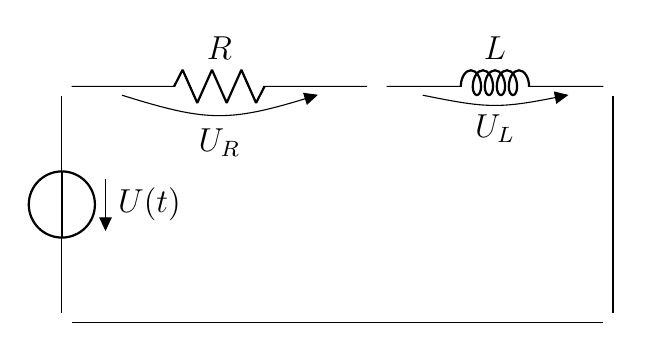
\begin{tikzpicture}[
  font=\large,
  every node/.style={font=\large}
]
  % Draw the circuit: voltage source -> R -> L -> back
  % Nodes
  \node (A) at (0,0) {};
  \node (B) at (0,3) {};
  \node (C) at (4,3) {};
  \node (D) at (7,3) {};
  \node (E) at (7,0) {};

  % Voltage source: draw from B (top) to A (bottom) without invert
  % => + at B (FROM-node, top), v-arrow points toward A (downward)
  % => matches KVL U(t) - U_R - U_L = 0
  \draw (B) to[V, v=$U(t)$] (A);

  % Top wire: R then L
  \draw (B) to[R, l=$R$, v=$U_R$] (C);
  \draw (C) to[L, l=$L$, v=$U_L$] (D);

  % Right wire down
  \draw (D) -- (E);

  % Bottom wire back
  \draw (E) -- (A);

\end{tikzpicture}
\end{document}
